
%(BEGIN_QUESTION)
% Copyright 2013, Tony R. Kuphaldt, released under the Creative Commons Attribution License (v 1.0)
% This means you may do almost anything with this work of mine, so long as you give me proper credit

\noindent
{\bf Capstone Assessment} (end of quarter)

\vskip 10pt

This performance assessment tests your mastery of many important instrumentation concepts.  You are to build a complete measurement and control loop (consisting of a transmitter, controller, and final control element), sketch an accurate loop diagram of the system, and demonstrate the ``automatic'' operation of the controller by stimulating the transmitter and noting the final control element's response.  All this must be done individually with no assistance from the instructor or from classmates, within one lab session (not to exceed three hours).  You may refer to manufacturer documentation and/or textbooks, but not to personal notes, while building your loop.  Your loop does not need to control a real process -- all it has to do is make a final control element respond automatically to a change in measurement.

You may perform the assessment activity at any time in the quarter.  Successful completion counts as the ``mastery'' portion of the course exam(s).  If you do not pass, the instructor will work with you to correct the problem(s).  There is no grade penalty for repeated attempts, however successful completion is required to pass the course.

\vskip 10pt

\noindent
{\bf Core elements} -- Your loop must contain, at minimum:

\begin{itemize}
\item{} A final control element consisting of a control valve (with positioner if you've passed the {\it INST250} course) or a variable-speed motor drive ({\it student's choice}).
\vskip 5pt
\item{} A 4-20 mA, loop-powered transmitter, either pressure or temperature -- RTD or thermocouple ({\it instructor's choice}).
\vskip 5pt
\item{} A single-loop controller, PLC loop controller, DDC controller, or DCS controller; either direct or reverse action ({\it instructor's choice}).
\end{itemize}

\vskip 10pt

\noindent
{\bf Additional elements} -- You will be required to demonstrate proficiency in the following details according to all Instrumentation courses you have cumulatively passed:

\begin{itemize}
\item{} If you have passed the {\it INST230} course \underbar{and} have chosen a motor drive as your FCE, you {\bf must} configure it for a speed (frequency) range selected by the instructor.
\vskip 5pt
\item{} If you have passed the {\it INST241} course, your transmitter and controller {\bf must} be accurately calibrated and ranged to register the process variable within $\pm$ 1\% of span accuracy.
\vskip 5pt
\item{} If you have passed the {\it INST250} course \underbar{and} have chosen a valve as your FCE, you {\bf must} use a positioner ranged to either 4-20 mA, 4-12 mA, or 12-20 mA as selected by the instructor.
\vskip 5pt
\item{} If you have passed the {\it INST251} course, you {\bf must} demonstrate either Proportional action, Integral action, or Derivative action as selected by the instructor.
\vskip 5pt
\item{} If you have passed the {\it INST262} course series, you {\bf must} use a networked controller and demonstrate how to operate the controller remotely from a personal computer.  On a control system where a personal computer is the normal operator interface (e.g. DDC, DCS), you must use ``remote access'' software such as RealVNC or Microsoft Remote Desktop from a different computer.
\end{itemize}

\vskip 10pt

Given the time constraint of this assessment, you will not be required to cut and fit flexible conduit to the field instruments.  All other wiring must be neatly installed so as to avoid creating safety hazards (tripping, etc.) and confusion for other students assembling their loops.

Limited availability of components and physical space in the lab means that only a few students will be able to work on this assessment at once, so plan on attempting this {\it well before} the final due date!

\vfil \eject

\noindent
{\bf Please follow these steps in order!}

\begin{itemize}
\item{} Approach the instructor to select the FCE and transmitter types.  {\bf You must work independently from now until project completion!}  You will wear a construction vest to alert classmates they are not to assist you, and to give you priority access to limited resources (e.g. computer workstations, calibration bench).
\vskip 10pt
\item{} If you are given your choice of transmitters, you should now select one and verify its proper function.  The purpose of this check is so you don't waste any of your three hours troubleshooting a faulty transmitter.  If this is a smart transmitter, now is a great time to digitally trim the sensor and output so that you merely have to re-range the transmitter during the 4-hour time limit (prerequisite: {\it INST241} course).  Alternatively, the instructor may assign a specific transmitter to you.
\vskip 10pt
\item{} Instructor makes all remaining selections: label your transmitter, controller, and FCE so no one disconnects them while you are building your loop.  {\bf You now have three hours to complete the loop!}  Instructor verifies that neither your controller nor FCE is pre-wired or pre-tubed.
\vskip 10pt
\item{} Sketch a loop diagram showing component wiring.  Present this to the instructor, who will check your planned circuit for errors.  The purpose of this step is to ensure you won't damage anything by incorrect wiring.  {\bf You are not allowed to begin wiring until the diagram has been approved, and you are not allowed to deviate from the diagram once approved!}
\vskip 10pt
\item{} Begin wiring your loop, keeping your wiring neat enough to not be a snag or trip hazard.
\vskip 10pt
\item{} Range your transmitter and controller to display the proper process variable range, so that the controller display reads precisely what the transmitter senses in real units (not just in percent), and configure the controller for the specified control action (direct or reverse).  Adjust the P, I, and D controller parameters to clearly demonstrate the selected control action (prerequisite: {\it INST251} course).
\vskip 10pt
\item{} Connect and configure the final control element within the loop.  If using a VFD, configure the acceleration and deceleration ramp times to 5 seconds each for relatively fast response, and set the speed range (prerequisite: {\it INST230} course).  If using a valve positioner, configure the positioner for the specified range (prerequisite: {\it INST250} course).
\vskip 10pt
\item{} Test the operation of the loop as a whole, and troubleshoot if necessary.
\vskip 10pt
\item{} Alert the instructor for a calibration check.  The instructor will input random values at your transmitter while you read the controller's display, checking for accurate correspondence (prerequisite: {\it INST241} course).
\vskip 10pt
\item{} Demonstrate to the instructor how to manipulate the final control element using the controller's ``manual'' mode.  The instructor will verify FCE range at this point (prerequisite: {\it INST230/250} course).
\vskip 10pt
\item{} Manually set the controller output to mid-range ($\approx$ 50\%), then switch to automatic mode to let the instructor test your controller's response for proper direction (direct or reverse) and control action (Proportional, Integral, or Derivative) (prerequisite: {\it INST251} course).  If you have passed {\it INST262}, you must remotely access your controller through a personal computer.
\vskip 10pt
\item{} {\bf Your loop is now complete.  The timed portion of the exercise is over.}
\vskip 10pt
\item{} Disconnect all signal and control wires (not the 120 VAC power wires, though) from all instruments and terminal blocks, as well as all pneumatic tubes.  Re-set the controller to its original configuration (0-100\% input range, gain = 1, integral and derivative actions off).  Show this to the instructor, and submit your loop diagram.
\vskip 10pt
\item{} Place calibration tag on transmitter and return it to storage.
\end{itemize}

\vskip 10pt


\vfil \eject

\noindent
\centerline{{\bf Capstone project check-list (listed in sequential order)} \hskip 50pt Name: \underbar{\hskip 80pt}}

\vskip 10pt

Remember that you must work \underbar{independently} to complete your loop once the instructor assigns you a vest to wear.  Any consultation with classmates, use of personal notes, or deviation from your loop diagram sketch (after instructor approval) will result in disqualification, which means you must take everything apart and begin anew (with difference selections).  You are allowed to use manufacturer documentation, as well as any documentation provided by the instructor (e.g. textbooks).

\vskip 20pt

\centerline{\bf No teamwork is allowed while wearing the vest!}

\vskip 10pt

% No blank lines allowed between lines of an \halign structure!
% I use comments (%) instead, so that TeX doesn't choke.

$$\vbox{\offinterlineskip
\halign{\strut
\vrule \quad\hfil # \ \hfil & 
\vrule \quad\hfil # \ \hfil \vrule \cr
\noalign{\hrule}
%
% First row
{\bf Selection} & {\bf (Circle/check)} \cr
%
\noalign{\hrule}
%
% Another row
You select FCE type & {\it Valve / Motor drive} \cr
%
\noalign{\hrule}
%
% Another row
Instructor selects transmitter & {\it Pressure / Temperature} \cr
%
\noalign{\hrule}
%
% Another row
Instructor assigns you a vest to wear &  \cr
%
\noalign{\hrule}
%
% Another row
You test the transmitter &  \cr
%
\noalign{\hrule}
} % End of \halign 
}$$ % End of \vbox

\vskip 10pt

\centerline{\bf The time clock starts now! \hskip 50pt Start time: \underbar{\hskip 80pt}}

% No blank lines allowed between lines of an \halign structure!
% I use comments (%) instead, so that TeX doesn't choke.

$$\vbox{\offinterlineskip
\halign{\strut
\vrule \quad\hfil # \ \hfil & 
\vrule \quad\hfil # \ \hfil \vrule \cr
\noalign{\hrule}
%
% First row
{\bf Step} & {\bf (Instructor writes/checks)} \cr
%
\noalign{\hrule}
%
% Another row
Instructor specifies transmitter range ({\it INST241 only}) &  \cr
%
\noalign{\hrule}
%
% Another row
Instructor specifies FCE range ({\it INST230/250 only}) &  \cr
%
\noalign{\hrule}
%
% Another row
Instructor selects controller -- {\bf label with your name!} &  \cr
%
\noalign{\hrule}
%
% Another row
Instructor selects direct/reverse controller action & \cr
%
\noalign{\hrule}
%
% Another row
Instructor selects P, I, or D action ({\it INST251 only}) &  \cr
%
\noalign{\hrule}
%
% Another row
Instructor selects FCE -- {\bf label with your name!} &  \cr
%
\noalign{\hrule}
%
% Another row
Instructor verifies nothing is pre-wired or pre-tubed &  \cr
%
\noalign{\hrule}
%
% Another row
You sketch loop diagram -- instructor verifies correctness &  \cr
%
\noalign{\hrule}
} % End of \halign 
}$$ % End of \vbox

\vskip 10pt

\centerline{\bf Now you may begin wiring and configuring the components}

% No blank lines allowed between lines of an \halign structure!
% I use comments (%) instead, so that TeX doesn't choke.

$$\vbox{\offinterlineskip
\halign{\strut
\vrule \quad\hfil # \ \hfil & 
\vrule \quad\hfil # \ \hfil \vrule \cr
\noalign{\hrule}
%
% First row
{\bf Step} & {\bf (Instructor checks)} \cr
%
\noalign{\hrule}
%
% Another row
Instructor verifies transmitter response (indicated at controller) &  \cr
%
\noalign{\hrule}
%
% Another row
Instructor verifies FCE response (controller in manual mode) &  \cr
%
\noalign{\hrule}
%
% Another row
Instructor observes automatic controller action (remotely, if applicable) &  \cr
%
\noalign{\hrule}
} % End of \halign 
}$$ % End of \vbox

\vskip 10pt

\centerline{\bf The time clock stops now! \hskip 50pt Stop time: \underbar{\hskip 80pt}}


% No blank lines allowed between lines of an \halign structure!
% I use comments (%) instead, so that TeX doesn't choke.

$$\vbox{\offinterlineskip
\halign{\strut
\vrule \quad\hfil # \ \hfil & 
\vrule \quad\hfil # \ \hfil \vrule \cr
\noalign{\hrule}
%
% First row
{\bf Step} & {\bf (Instructor checks)} \cr
%
\noalign{\hrule}
%
% Another row
Instructor verifies all signal wires/tubes disconnected &  \cr
%
\noalign{\hrule}
%
% Another row
Instructor verifies controller reset to original configuration &  \cr
%
\noalign{\hrule}
%
% Another row
Instructor verifies transmitter is tagged and stored &  \cr
%
\noalign{\hrule}
%
% Another row
Instructor collects your loop diagram &  \cr
%
\noalign{\hrule}
} % End of \halign 
}$$ % End of \vbox

\vskip 10pt

\centerline{\bf Your mastery score will not be recorded until \underbar{all} steps are complete!}







\vfil \eject

\centerline{\bf Notes on instrument ranging}

\vskip 10pt

An important criterion for the capstone project is that the loop instruments be properly ranged.  For students who have completed the INST241 course, this means both the transmitter and controller must be accurately calibrated and ranged to register the process variable within $\pm$ 1\% of span accuracy, so that any stimulus (e.g. pressure, temperature) input to the transmitter will be faithfully registered on the controller's faceplate display.  For students choosing final control elements related to courses they have completed (i.e. VFD motor drives for INST230 or pneumatic control valves for INST250), that final control element must respond to the loop controller's output signal with an appropriate range.

\vskip 10pt

The reason this is an issue at all is because loop controllers operating on 4-20 mA analog signals don't ``know'' what those signals are supposed to represent unless someone configures the controller with the proper range reflecting real-world conditions.  For example, if a student is assigned a temperature transmitter with a range of 300 to 800 degrees Fahrenheit, not only does the transmitter have to output 4 mA when sensing 300 $^{o}$F and output 20 mA when sensing 800 $^{o}$F, but the controller must display an indication of 300 $^{o}$F when it receives a 4 mA signal from the transmitter, and display an indication of 800 $^{o}$F when it receives a 20 mA signal from the transmitter.  None of this happens on its own -- the student must range the transmitter for 300-800 $^{o}$F input (and 4-20 mA output) as well as range the controller to display 300-800 $^{o}$F over its 4-20 mA input scale.  A typical loop is shown here with all instrument ranges displayed:

$$\includegraphics[width=15.5cm]{i02499x01.eps}$$

Analog (non-``smart'') transmitters, I/P transducers, and valve positioners are ranged using ``zero'' and ``span'' adjustments, typically screws or nuts.  The ranging of analog instruments is discussed in the ``Instrument Calibration'' chapter of the {\it Lessons In Industrial Instrumentation} textbook.

\vskip 10pt

Digital (``smart'') transmitters and valve positioners are ranged by setting LRV and URV parameters using a ``communicator'' device or a personal computer equipped with the appropriate interface and software.  This too is discussed in the ``Instrument Calibration'' chapter of the {\it Lessons In Industrial Instrumentation} textbook. 

\vskip 10pt

\filbreak

Digital electronic loop controllers similarly provide means to set the range values for interpreting any 4-20 mA signal input to them.  Exactly what these parameters are called and how they are accessed varies from one model and brand of loop controller to another.  Here are some examples:

\begin{itemize}
\item{} Siemens/Moore 352 controller: process variable range parameters are located in the ``Operator's Display'' function block (FB15):
\begin{itemize}

\item{} URV = {\it Process Hi}
\vskip 10pt
\item{} Siemens/Moore 352P and 353 controller: process variable range parameters are located in the ``Analog Input'' function block (AIN):
\begin{itemize}

\item{} URV = {\it Maxscale}
\vskip 10pt
\item{} Emerson DeltaV DCS: process variable range parameters are located in the ``Analog Input'' function block (AI) and ``PID'' function block (PID), both conforming to the FOUNDATION Fieldbus standard.  This standard for function block configuration is adhered to in the DeltaV system even if the loop in question uses analog (4-20 mA) signals.  Detailed information may be found in any FOUNDATION Fieldbus function block reference manual:
\begin{itemize}

\item{} (PID block) = the {\it PV\_SCALE} parameter contains both high and low range limits, engineering units (e.g. deg F), and decimal point position.
\vskip 10pt
\item{} Honeywell UDC 2500 controller: process variable input \#1 range parameters are located in the ``Input 1'' set-up group of parameters:
\begin{itemize}

\item{} URV = {\it IN1 HI}
\vskip 10pt
\item{} Automation Direct ``SOLO'' controller: process variable range parameters are located in the following registers:
\begin{itemize}

\item{} URV = {\it P3-3 Input Range High}
\vskip 10pt
\item{} Allen-Bradley PLC5, SLC500, and MicroLogix controllers: process variable scaling parameters are typically located either in a ``Scale'' instruction (SCL) or a ``Scale with Parameters'' instruction (SCP).  In either case, the instruction takes the raw count value from the input channel's analog-to-digital converter and scales it into the desired process variable display range.  A YouTube video on our BTCInstrumentation channel shows how to do this for the networked MicroLogix PLCs in the lab:
\begin{itemize}

\item{} (SCP instruction LRV) = {\it Scaled Min.}
\item{} (SCP instruction URV) = {\it Scaled Max.}
\vskip 10pt
\item{} Allen-Bradley Logix5000 controller: process variable scaling parameters are located in the ``PID'' instruction (PID):
\begin{itemize}

\item{} URV = {\it .MAXS}
\end{itemize}
\end{itemize}

\vskip 10pt

Output ranging is typically done in the final control element itself: within the VFD in the case of a motor drive, and within the positioner in the case of a pneumatic control valve.




\underbar{file i02499}
%(END_QUESTION)





%(BEGIN_ANSWER)

The only ``answer'' to this question is a properly documented and functioning instrument loop!

%(END_ANSWER)





%(BEGIN_NOTES)


%INDEX% Capstone assessment: end-of-quarter demonstration of instrument loop (LEGACY)

%(END_NOTES)


